\section{Description and Methodology}

\subsection{Compiling the Linux kernel}
We were supplied with a variant of Linux called \emph{uClinux}, and it's supplied toolchain. We built the distribution by using a build system named \emph{ptxdist}. We followed \cite[section 5.3]{compendium} step by step, and when done we ended up with a working linux distribuion on the chip, with Tux drawn on the screen. Initially we did not change the kernel config\footnote{We ended up doing so, please see section \ref{subsection:energy-efficiency}.}, nor add any more packages than already configured.

\subsection{Device driver for the gamepad}

\subsection{Signals and interrupts}
\label{subsection:signals-and-interrupts}

\subsection{Controlling the framebuffer device}
The EFM32GG has it's own framebuffer device that manages the display. This device is accessed by opening the driver \emph{/dev/fb0} as a file. When the file is opened, we have access to the drivers methods. As described in \cite[section 5.4.2]{compendium}, this means that we can use \emph{read()}, \emph{write()} and \emph{lseek()} wich can be used to handle the frambuffer byte by byte as a usual file. But, as \cite[section 5.4.2]{compendium} describes, there is a way controlling the frambuffer that is easier and faster then using the mentioned method. \\

The framebuffer divice can be memory mapped. This means that we can map the driver to an array in memory, which in C means that we are able to write pixels directly with an usual C array. This done by calling the function \emph{mmap()}, wich is a Unix system call defined in the header \emph{sys/mmap.h}. 
Writing to the array will update a buffer holding the pixel values. To write the changes in the framebuffer to the display we use the system call \emph{ioctl()}. \\

\emph{ioctl()} is driver specific system call, and can be used to a various of tasks. In our case, it is to update the changes in the framebuffer. The number of parameters to this function varies depending on the driver, but it needs two parameters to work properly. The first is an file descriptor for an open file. The second, a device dependent request code wich specifies if it is an \emph{in} or \emph{out} parameter, and the size of the list of driver specific parameters in bytes. See \footnote{http://man7.org/linux/man-pages/man2/ioctl.2.html} for more information.   
\\

After we are done using the display, it is important to clean up. First we have to undo the memory mapping, wich is done by calling the system call \emph{munmap()} (defined in \emph{sys/mmap}). Second we have to close our connection to the device, wich is done by calling \emph{close()} to the framebuffer driver. \\

Our module \emph{screen.c} is responsible of handling the framebuffer device. We memory map the frambuffer in the module. The module contains methods to initialize the display and close the connection to the device, by calling the functions described in this section. It also contains methods to draw simple elements to the screen, in various ways. See the code for more information. 

\subsection{Pong}

\subsection{Energy efficiency}
\label{subsection:energy-efficiency}
As we are no longer programming on the "bare metal", we have less control over the software running on the chip. \emph{uClinux} have certain requirements regarding timers and other peripherals, and \cite{compendium} states that "all relevant clocks are already turned on", which we consider as a statement that says the oscilator setup is fixed, and should not be altered for this exercise.

\subsubsection{Interrupts and signals}
We implemented our driver so no polling mechanisms were needed (as described in section \ref{subsection:signals-and-interrupts}). As a consequence, the program will stay most of its time in a \emph{pause()} loop, leaving the CPU and IO buses free to do other stuff, or in this case, sleep. This behaviour decreases power consumption.

\subsubsection{Optimizing screen update}


\subsubsection{Tickless idle}
\begin{figure}[h]
	\centering
	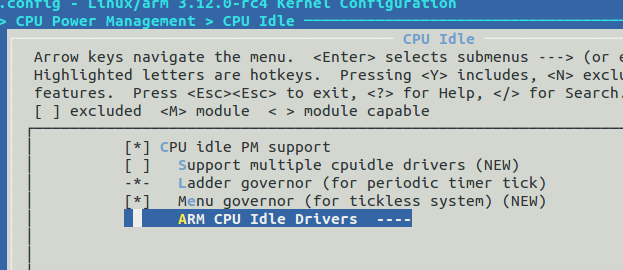
\includegraphics[width=12cm]{img/tickless.png}
	\caption{Configuring the kernel to tickless idle}
	\label{fig:tickless}
\end{figure}
Because our game is handeled entirely by signal handlers, leaving the main program in a pause loop, we wanted to reduce the power consumption while waiting for an interrupt/signal. In order to do that, we were adviced to put the kernel in a mode known as tickless idle. We did this by setting
